%!TEX root = main.tex

\begin{figure*}[tbp]
	\newcommand\mywidth{0.26}
	\centering
	\subfloat[] {
		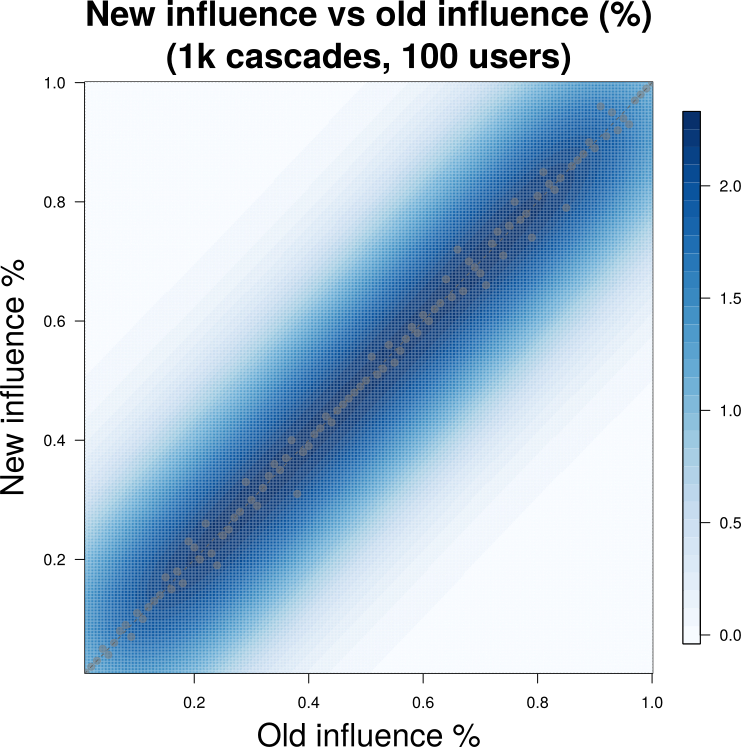
\includegraphics[height=\mywidth\textheight]{1-simulated-data}
		\label{si-fig:new-old-simulated}
	}
%	\hspace{0.15cm}
	\subfloat[] {
		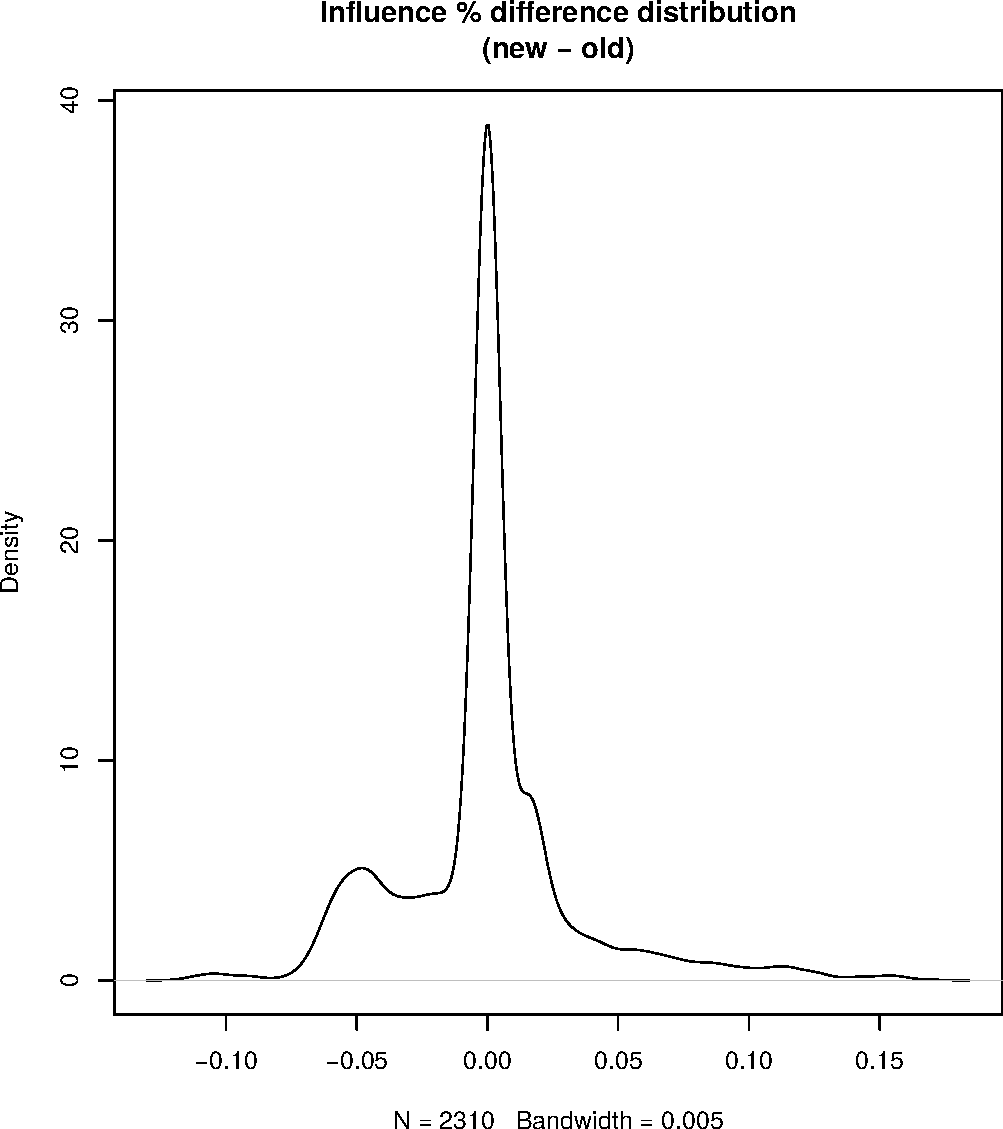
\includegraphics[height=\mywidth\textheight]{2-real-data-diff}
		\label{si-fig:new-old-real-diff}
	}
%	\hspace{0.15cm}
	\subfloat[] {
		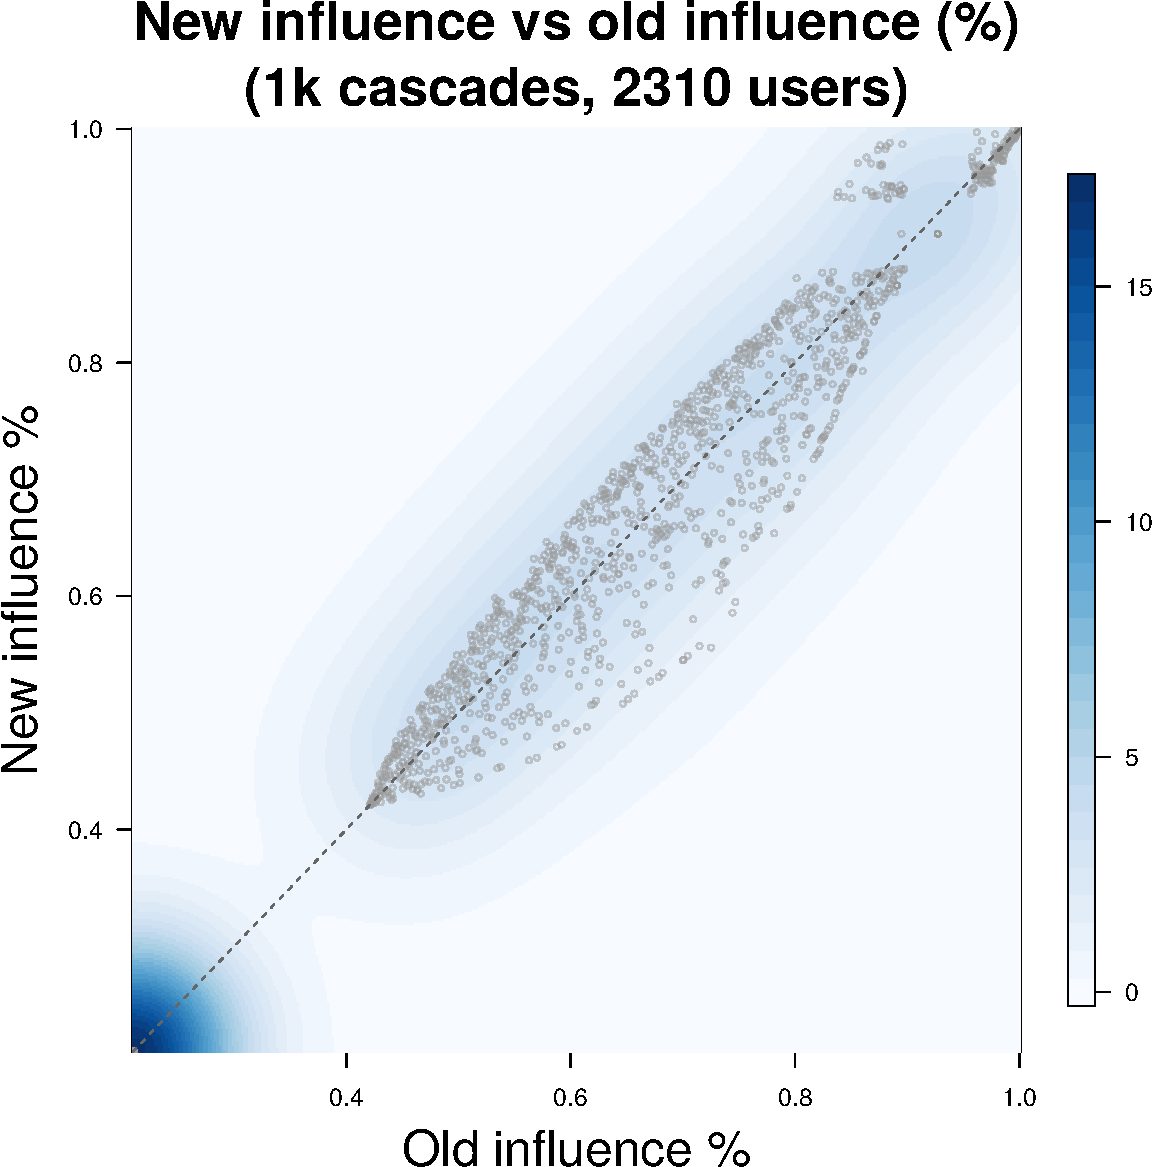
\includegraphics[height=\mywidth\textheight]{3-real-data-2d-plot}
		\label{si-fig:new-old-real}
	}
	\caption{
		Wordclouds of partisan hashtags in \debate: Democrat \textbf{(top)} and Republican \textbf{(bottom)}.
		Hashtags sizes are scaled by their frequency.
	}
	\label{fig:wordclouds}
%	\captionmoveup
\end{figure*}